\documentclass[usletter]{article}
\usepackage{DejaVuSans}
\renewcommand*\familydefault{\sfdefault}
\usepackage[T1]{fontenc}
\usepackage{graphicx}
\usepackage{listings}
\usepackage{pdfpages}
\usepackage{multirow}
\usepackage{lscape}
\usepackage{graphics}
\usepackage{longtable}
\usepackage{graphics}
\usepackage{lscape}
\usepackage[hidelinks]{hyperref}
\begin{document}

  \begin{titlepage}
  \begin{center}

  {\Huge Open Game Module}

  \vspace{25mm}

  
\includegraphics[width=0.90\textwidth,height=\textheight,keepaspectratio]{img/SPARKLETRON.png}

  \vspace{25mm}

  \today

  \vspace{15mm}

  {\Large Jay Convertino}

  \end{center}
\end{titlepage}

\tableofcontents

\newpage

\section{Introduction}

\par
Open Game Module is a open source expansion card for the Colecovision. This module is Super Game Module (SGM) compatable.
This means all SGM games will run when this module is used with a Colecovision. The sound is expanded with a Yamaha YMZ284
instead of the GI AY chip.

\subsection{Fix for opcode games}

Opcode super game module mega cart games have a particular check for the sound chip in there startup routine.

\begin{enumerate}
  \item Set AY register address to 0x00
  \item Write the value 0xAA to AY (register 0x00).
  \item Set AY register address to 0x02
  \item Write the value 0x55 to AY (register 0x02).
  \item Set AY register address to 0x00
  \item Read the value from AY (register 0x00).
  \item Compare to value originally written (0xAA), fail if not matching
  \item Set AY register address to 0x02
  \item Read the value from AY (register 0x02).
  \item Compare to value originally written (0x55), fail if not matching.
\end{enumerate}

The hack fix for my setup is to only have 4 8 bit regiters for 0,1,2,3,4,5,6, and 7. The mapping is
AY Software Register ADDRESS => Cache Register ADDRESS

\begin{itemize}
  \item 0 => 0
  \item 1 => 0
  \item 2 => 1
  \item 3 => 1
  \item 4 => 2
  \item 5 => 2
  \item 6 => 3
  \item 7 => 3
\end{itemize}

\subsection{Specifications}

\par
\begin{itemize}
  \item 32 KB of RAM
  \item YMZ284 Sound Chip
  \item MAX7000S CPLD (EPM7064SLC)
  \item PCB, two layer
\end{itemize}

\subsection{Parts List}

\subsubsection{electronics}
\begin{footnotesize}
\begin{longtable}{ |*{4}{c|} }
\hline
{Item} & {Qty} & {Reference(s)} & {Value} \\
\hline
{1} & {1} & {J1} & {Connector, 60 pin} \\
\hline
{2} & {4} & {C1, C2, C3, C4} & {100pF} \\
\hline
{3} & {1} & {U1} & {EPM7064SLC-10} \\
\hline
{4} & {1} & {U2} & {YMZ284} \\
\hline
{5} & {1} & {U3} & {HM62256BLP} \\
\hline
{6} & {1} & {R5} & {470R} \\
\hline
{7} & {1} & {R6} & {4k7} \\
\hline
{8} & {4} & {R1, R2, R3, R4} & {1k} \\
\hline
{9} & {1} & {J2} & {Pin Header, 10 pin} \\
\hline
\end{longtable}
\end{footnotesize}

\subsubsection{hardware}
\begin{footnotesize}
\begin{longtable}{ |*{4}{c|} }
\hline
{Item} & {Qty} & {Reference(s)} & {Value} \\
\hline
{1} & {4} & {S1} & {\#2-32 x 1/4 Fastenal 0148209, screw} \\
\hline
{2} & {1} & {TOP} & {top.stl 100.00} \\
\hline
{3} & {1} & {BOTTOM} & {bottom.stl 100.00} \\
\hline
\end{longtable}
\end{footnotesize}

\section{Building}

\par
This document assumes some Electrical Engineering knowledge. Building circuits is not
trivial due to the mix of SMD and through hole components. What follow are general
steps to build the Mini Colecovision

\begin{itemize}
  \item Create PCB from schematic/gerber/open\_game\_module.zip
  \item Populate PCB
  \item Power up and program CPLD
  \item Build your own case
\end{itemize}

\subsection{Directory Guide}

\par
Below highlights important folders from the root of the open\_game\_module.

\begin{enumerate}
  \item \textbf{docs} Contains all documentation related to this project.
    \begin{itemize}
      \item \textbf{datasheets} Contains all datasheets for components.
      \item \textbf{manual} Contains user manual and github page that are generated from the latex sources.
    \end{itemize}
  \item \textbf{img} Contains images of the project
  \item \textbf{schematic} KiCAD v8.X schematic and PCB designs
    \begin{itemize}
      \item \textbf{gerber} Contains gerber files and archives for production.
      \item \textbf{pdf} PDF schematic
    \end{itemize}
  \item \textbf{src} CPLD firmware source
    \begin{itemize}
      \item \textbf{open\_game\_module} Contains verilog source code and constraits
      \item \textbf{quartus13sp01} Quartus project used to generate firmware.
    \end{itemize}
\end{enumerate}

\subsection{Dependencies}

\par
The following are the dependencies needed to build the firmware and PCB for the system.

\begin{itemize}
  \item Quartus 13.0 sp1
  \item python 3.X
  \item KiCAD v8.X
\end{itemize}

\subsubsection{Open Game Module Glue File List}
\begin{itemize}
\item src
	\begin{itemize}
	\item {'src/open\_game\_module.v': {'file\_type': 'verilogSource'}}
	\end{itemize}
\item constr
	\begin{itemize}
	\item {'constr/open\_game\_module.sdc': {'file\_type': 'SDC'}}
	\end{itemize}
\item tb
	\begin{itemize}
	\item {'tb/tb\_open\_game\_module.v': {'file\_type': 'verilogSource'}}
	\end{itemize}
\end{itemize}


\subsubsection{Fusesoc}
\par
Fusesoc is used for the simulation target only. There are no build targets due to the use of Quartus 13.0sp1.
This makes the use of it a bit silly. It does make it easier to use in future projects where the RAM,ROM,CPU,VDP,
and Sound chips are also IP cores.

\subsubsection{Open Game Module Glue Targets}
\begin{itemize}
\item default
	\begin{itemize}
	\item[$\space$] Info: Default IP target for future tool intergration.
	\item src
	\item constr
	\end{itemize}
\item sim
	\begin{itemize}
	\item[$\space$] Info: Simulation target for basic test bench.
	\item src
	\item tb
	\end{itemize}
\end{itemize}


\subsubsection{Quartus}
\par
This project uses the last version of Quartus that supports the MAX7000S series. The version is 13.0sp1.
The project is located at src/quartus13sp01/. Once you have the project open please follow the softwares steps
for building and programming the CPLD bitfile.

\subsection{PCB}

\par
The top has all the components of the circuit.

\begin{figure}[h!]
\caption{Top}
\centering
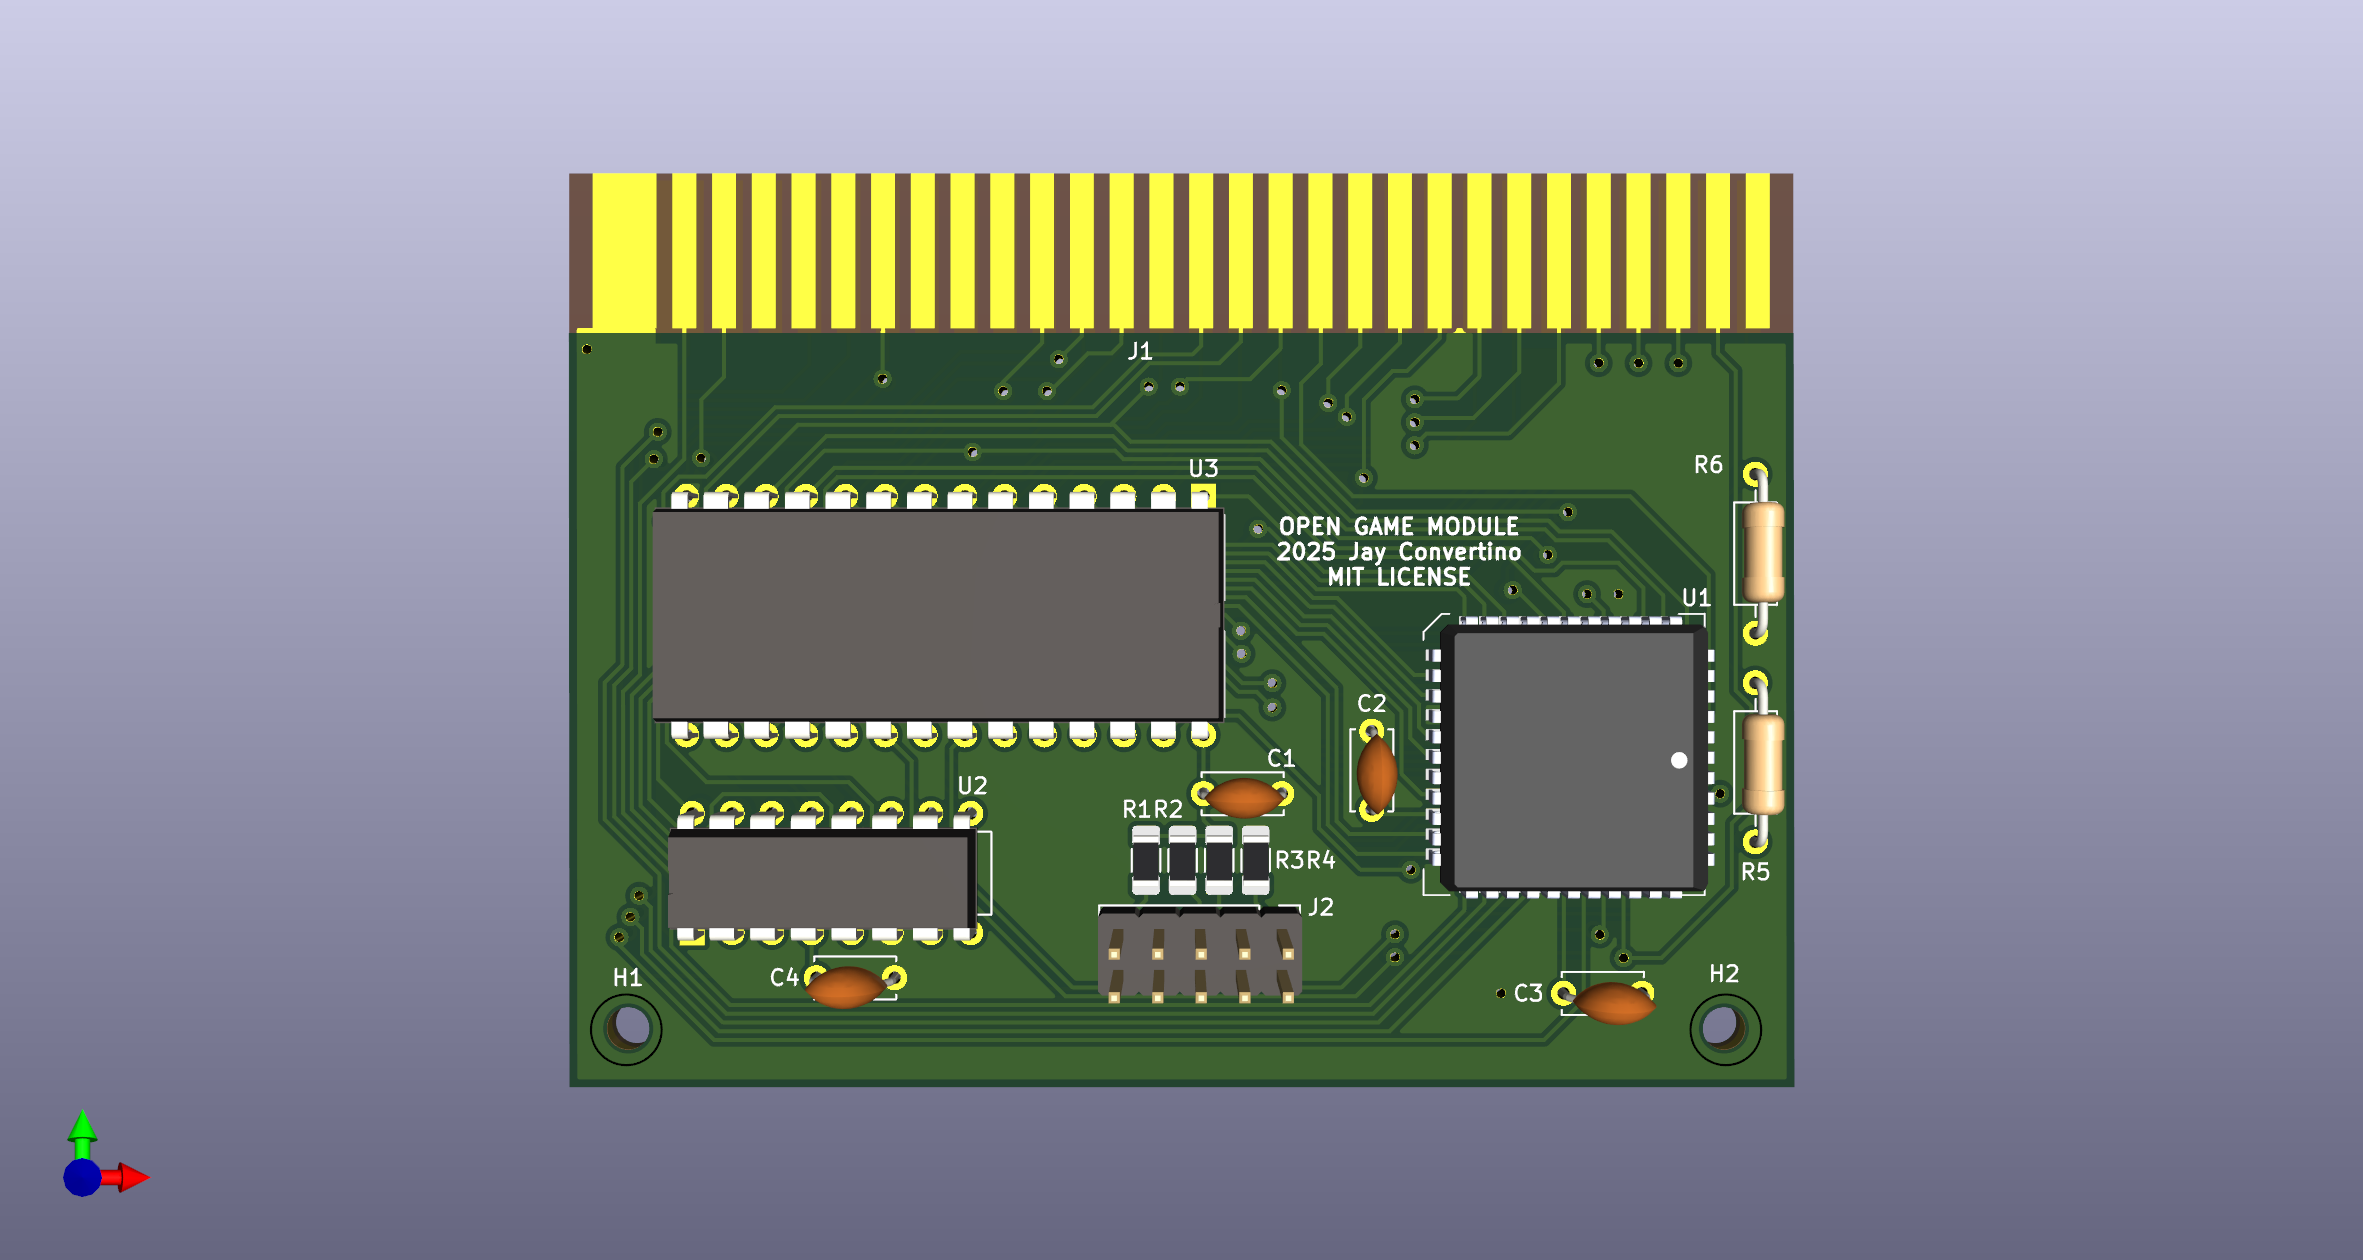
\includegraphics[width=0.90\textwidth,keepaspectratio]{img/ogm_top.png}
\end{figure}

\par
The bottom has no components.

\begin{figure}[h!]
\caption{Bottom}
\centering
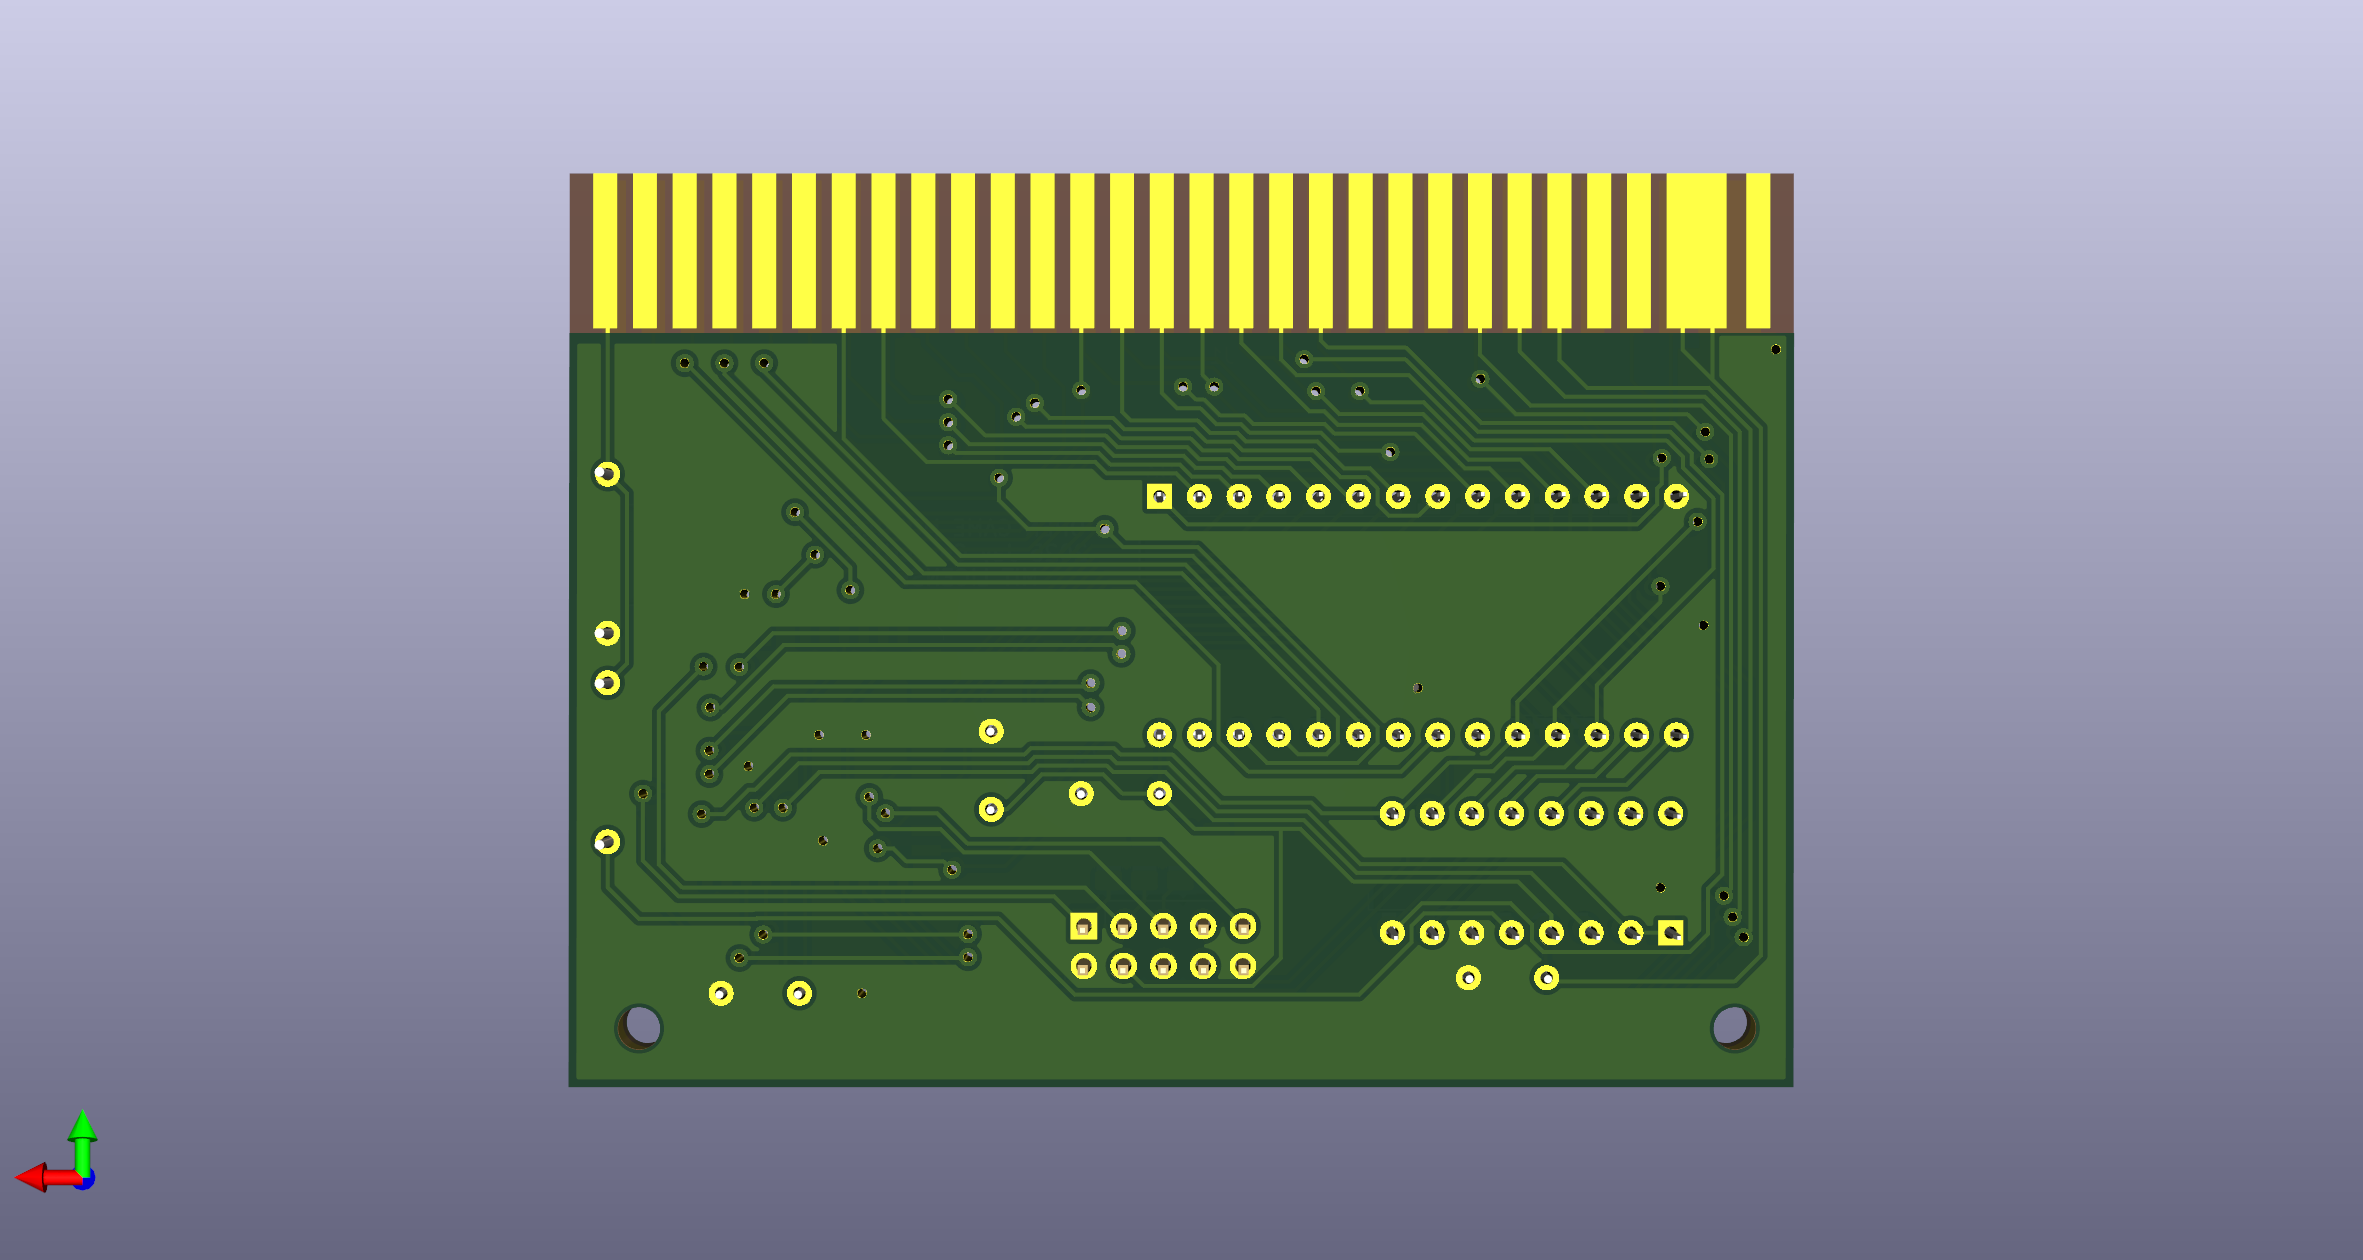
\includegraphics[width=0.90\textwidth,keepaspectratio]{img/ogm_bottom.png}
\end{figure}

\subsection{3D Printed Case}

\par
The 3D printed case has been tested on two different printers. It has only been tested with ABS filament.
The parts list for the 3D printed case has the STL file name in the value and the XXX.X value is the scale size.
In general I recommend the following steps for assembly.

\begin{enumerate}
  \item Bottom, sit pcb aligned to screw holes.
  \item Top, sit top half on top and install screws.
\end{enumerate}

\subsection{CPLD Programming}

\par
There is one device that need to be programmed which is the CPLD (complex programmable logic device).
This is programmed with quartus using the JTAG header to upload the bitfile.
\par
Quartus 13.0sp1 is the easiest way to build and program the MAX7000 CPLD. You will need an altera blaster.
I recommend the chinese clone blasters, they actually worked the best. While the worst was the Terasic blaster
which did not work at all. As for instructions on how to program it in Quartus, please see the software for details.

\newpage

\section{Usage}

\subsection{Console}
\par
The expansion module must be firmly inserted into the expansion connector of the Colecovision. If you have issues, be sure
to clean the connectors.

\begin{enumerate}
  \item \textbf{Open Expansion Cover} 
\includegraphics[width=0.50\textwidth,keepaspectratio]{img/SPARKLETRON.png}
  \item \textbf{Insert Open Game Module} 
\includegraphics[width=0.50\textwidth,keepaspectratio]{img/SPARKLETRON.png}
\end{enumerate}

\subsection{Software Programming}
\par
Module Documentation has in\-depth details for using the open game module and register bits. You could do this in many different ways, but
having the SDCC compiler know ahead of time that the RAM is there works well for me. There are different stragies that could be done for this
but I feel this is the simplest way. Other methods can provide better detection of the OGM. The psudo code steps are as follows.

\begin{enumerate}
  \item Setup expansion RAM, (NOTE COULD CHECK IF REGISTER VALUE IS EQUAL TO THE DEFAULT TO VERIFY SGM)
  \item Setup IRQS
  \item Copy IRQs to RAM where ROM jumps used to be.
  \item Setup Sound CHIP, (READ BACK TO CHECK EXISTANCE)
\end{enumerate}

\subsubsection{Assembly Code For RAM Init}

\par
This brief assembly code doesn't actually check for the SGM it simply enables the ram registers, sets the irqs, and starts main. This code is taken
from RODAC and isn't complete, see RODAC coleco\_sgm arch crt0.s for complete code. I does give a decent idea on how to set the SGM registers for RAM.

\begin{lstlisting}[language={[x86masm]Assembler}]
_SGM_RAM_ENA_PORT     .equ 0x0053
_SGM_BIOS_SWAP_PORT   .equ 0x007F
_NMI_SIZE             .equ (_irq_nmi_end - _irq_nmi + 1)
_SPIN_SIZE            .equ (_irq_spin_end - _irq_spin + 1)
;setup for super game module.
ld a,#0x01
out (_SGM_RAM_ENA_PORT), a
ld a,#0x0D
out (_SGM_BIOS_SWAP_PORT), a
;setup ram locations with irq vectors?, 0x8 etc.
;reti
ld a,#0xED
ld (0x08),a
ld (0x10),a
ld (0x18),a
ld (0x20),a
ld (0x28),a
ld (0x30),a
ld a,#0x4D
ld (0x09),a
ld (0x11),a
ld (0x19),a
ld (0x21),a
ld (0x29),a
ld (0x31),a
;copy code to ram
;nmi first
ld bc, #_NMI_SIZE
ld hl, #_irq_nmi
ld de, #0x0066
ldir
;spin
ld bc, #_SPIN_SIZE
ld hl, #_irq_spin
ld de, #0x0038
ldir
ld	sp, #0x8000
call gsinit
call  _main
rst   0x0
\end{lstlisting}

\subsubsection{C Code for SDCC}

\par
The code below is based on using SDCC 4.X.X as the C complier with a custom crt0.s. Essentially for the sound chip you
need to communicate with it by writing to the ports a address, then the data. You can also read from the ports to
verify the chip exists and that the OGM is working. Though for the OGM its chip does not have a read function. It is
emulated for registers 0, 2, and 4 (0=1, 2=3, and 4=5) in the CPLD so all opcode/team pixelboy games will startup correctly.

\begin{lstlisting}[language=C]

#define GI_SND_CP_ADDR    0x50
#define GI_SND_WDATA_ADDR 0x51
#define GI_SND_RDATA_ADDR 0x52

__sfr __at(GI_SND_CP_ADDR)    GI_SND_CP_PORT;
__sfr __at(GI_SND_WDATA_ADDR) GI_SND_WDATA_PORT;
__sfr __at(GI_SND_RDATA_ADDR) GI_SND_RDATA_PORT;

/*** send address to chip ***/
inline void sendAddr(uint8_t addr)
{
  di();

  GI_SND_CP_PORT = addr;

  ei();
}

/*** send data to chip ***/
inline void sendData(uint8_t data)
{
  di();

  GI_SND_WDATA_PORT = data;

  ei();
}

/*** send data to chip ***/
inline void readData(uint8_t data)
{
  di();

  data = GI_SND_RDATA_PORT;

  ei();
}
\end{lstlisting}


  \section{Module Documentation}
  \par What follows are PDF pages generated from natural docs HTML pages. This documents
  the source code used for the CPLD.

  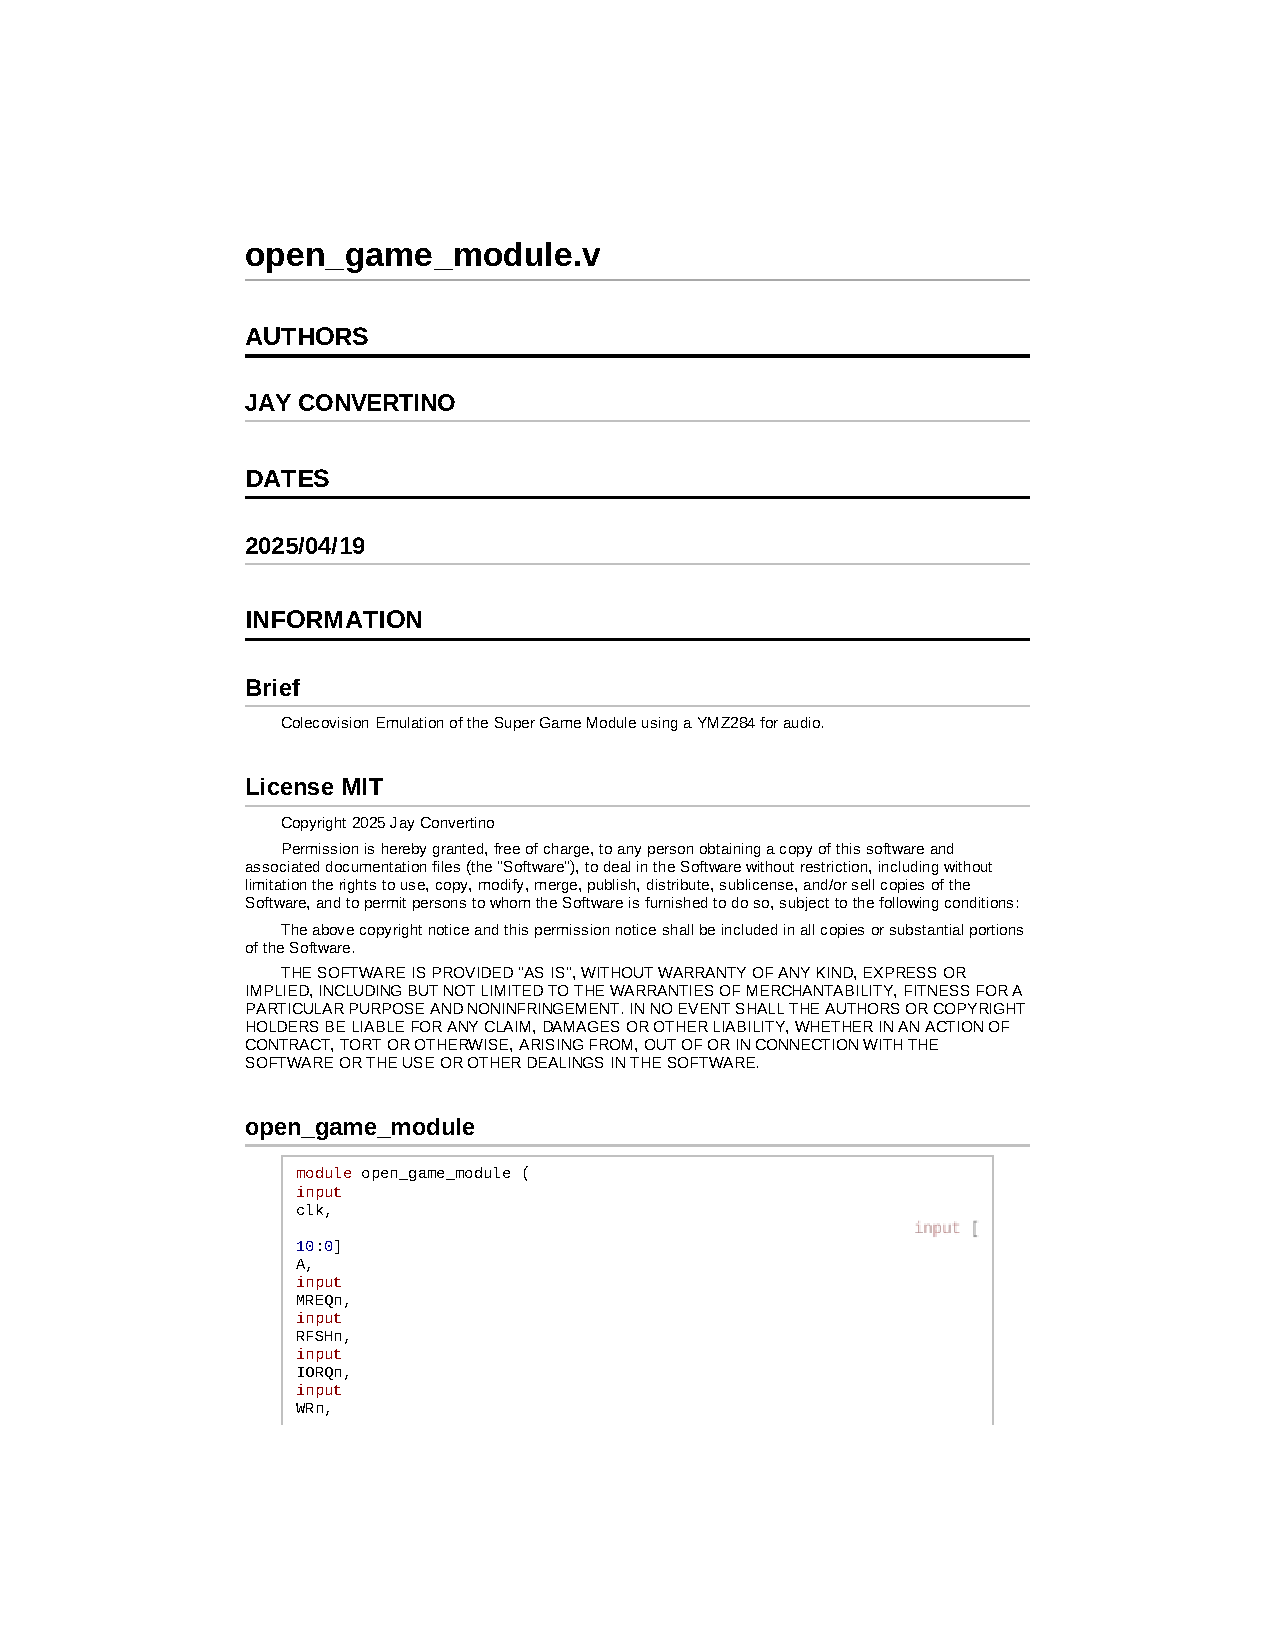
\includepdf[pages=-, addtotoc={1,subsection,1,Open Game Module,p1}, pagecommand={}]{open_game_module-v.pdf}

  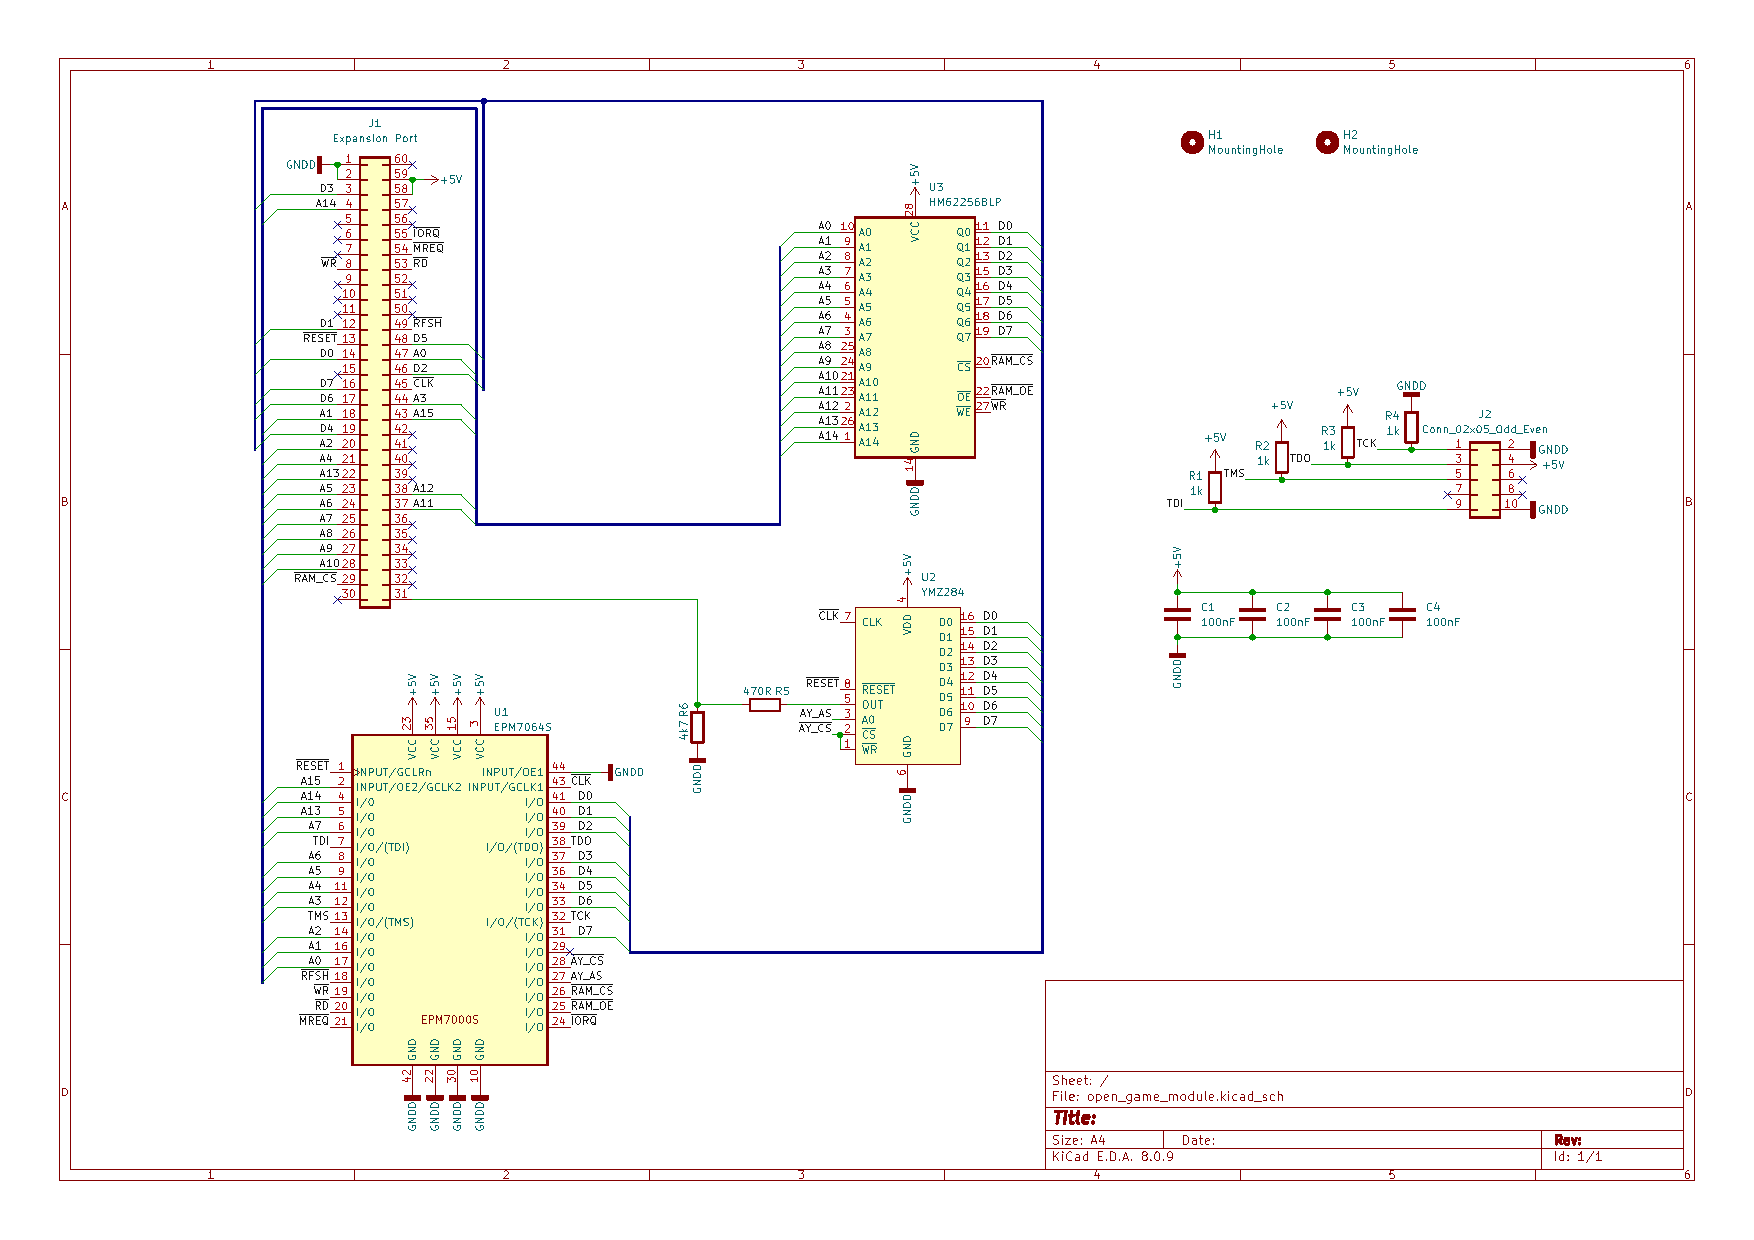
\includepdf[pages=-, addtotoc={1,subsection,1,Open Game Module,p1}, pagecommand={\section{Schematics}}]{../schematic/open_game_module.pdf}

\end{document}
